React components can go in four different of its life. 

\begin{itemize}
    \item \textbf{Initialization}: In this stage the component is constructed with the given \textbf{props} and default state. 
    This is done in the constructor of the component class. 
    \item \textbf{Mounting}: Is the stage of rendering the JSX returned by the render method itself.
    \item \textbf{Updating}: The stage the application state is updated and the application is repainted. 
    \item \textbf{Unmounting}: Is the final step where the component will be removed from the page. 
\end{itemize}



\begin{figure}[h]
\centering
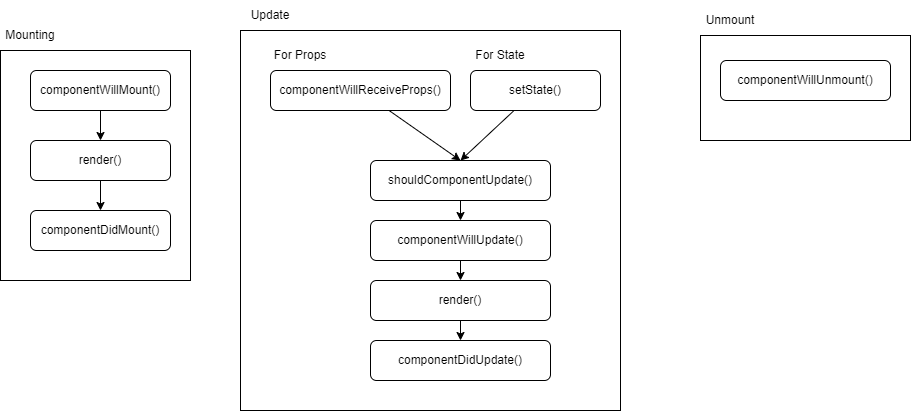
\includegraphics[width=1\linewidth]{figures/01_lifecycle.png}
\caption{React lifecycle}
\label{fig:lifecycle}
\end{figure}

https://www.geeksforgeeks.org/reactjs-lifecycle-components/

